\chapter{Supplementary Results}
%100 runs of 3 parameter sets
\begin{figure}[h!]
\centering
\noindent\code{Divergence Matrix}{results/HundredResults.txt}
\caption[Output file of ES1, ES2 comparison query.]{VI scores of ES1 and ES2 run with 3 distinct parameter sets (variations of omega) run on 100 repetitions. ES2 was more accurate for higher omega values.}
\label{fig:HundredResultsFile}
\end{figure}


\begin{figure}[h!]
  \centering
    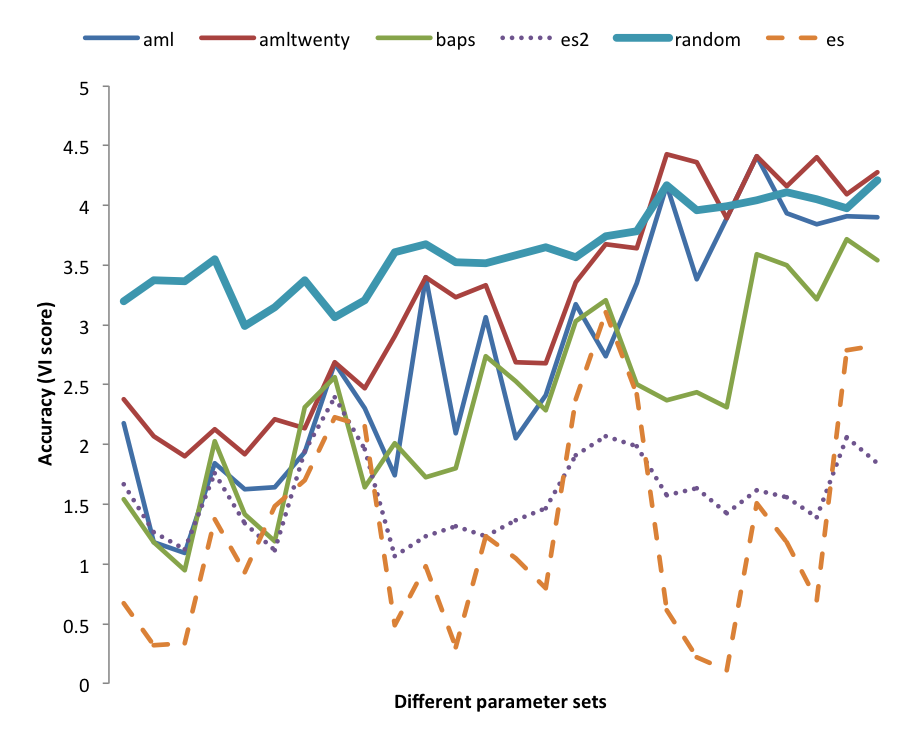
\includegraphics[scale=0.75]{images/ResultGraphs/ResultGraphs-3}
      \caption[All demarcation graphical accuracy visualization on $nu = 50$.]{Across 27 parameter set combinations I exhaustively test all demarcation programs on $npop$ values of 10, 20, and 30, $\Omega$ values of 0.019, 0.19, and 1.9, $\sigma$ values of 0.11, 1.1, and 11, for nu of 50 sequences. Random demarcation is represented by the solid line. On the $y$-axis we have VI scores, where values closer to 0 represent more accurate demarcation runs.}
    \label{fig:All50}
\end{figure}

\begin{table}
%    \begin{tabular}{l|ccccc}
%    ~                  & AdaptML     & AdaptML$^\ast$    & Baps        & Ecotype Simulation 2 & Random      \\ \hline
%    Average            & 2.767371639 & 3.185623443 & 2.359650359 & 1.589546505          & 3.631545086 \\
%    Standard Deviation & 0.971373851 & 0.868775294 & 0.783228066 & 0.34336826           & 0.34949857  \\
%    \end{tabular}
    \begin{tabular}{l|cc}
    ~                    & Average     & Standard Deviation \\ \hline
    AdaptML              & 2.767371639 & 0.971373851        \\
    $^\ast$AdaptML              & 3.185623443 & 0.868775294        \\
    BAPS                 & 2.359650359 & 0.783228066        \\
    ES 2 & 1.589546505 & 0.34336826         \\
    Random               & 3.631545086 & 0.34949857         \\
    \end{tabular}
    \caption[Statistics on all demarcators on $nu=50$.]{Statistics on all demarcators run with 5 reps on a dataset of $nu=50$. ($^\ast$) Represents AdaptML ran with a habitat specialization value of 20.}
        \label{tab:50Allmean}
\end{table}

\begin{figure}[h!]
  \centering
    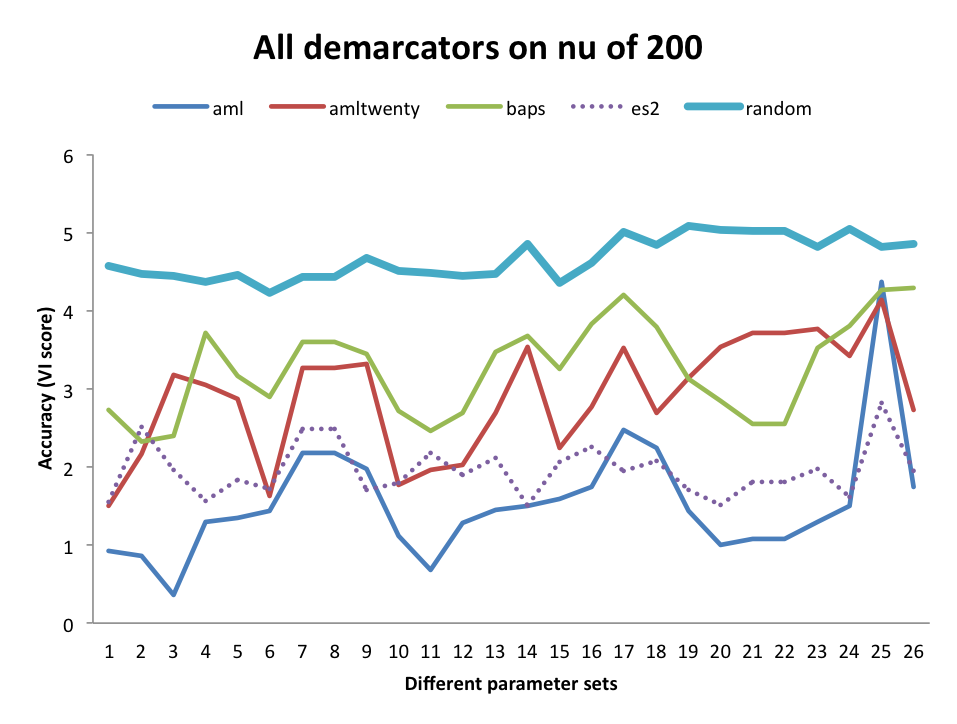
\includegraphics[scale=0.75]{images/ResultGraphs/ResultGraphs-1}
      \caption[All demarcation graphical accuracy visualization on $nu = 200$.]{Across 27 parameter set combinations I exhaustively test all demarcation programs on $npop$ values of 30, 40, and 50, $\Omega$ values of 0.019, 0.19, and 1.9, $\sigma$ values of 0.11, 1.1, and 11, for nu of 200 sequences. Random demarcation is represented by the solid line. On the $y$-axis we have VI scores, where values closer to 0 represent more accurate demarcation runs.}
    \label{fig:All200}
\end{figure}

\begin{table}
%    \begin{tabular}{l|ccccc}
%    ~                  & AdaptML     & AdaptML$^\ast$     & BAPS        & Ecotype Simulation 2 & Random      \\ \hline
%    Average            & 1.543424394 & 2.908133924 & 3.265003881 & 1.955714164          & 4.667531001 \\
%    Standard Deviation & 0.748104722 & 0.713876097 & 0.59283446  & 0.33348659           & 0.258112685 \\
%    \end{tabular}
\begin{tabular}{l|cc}
    ~                    & Average     & Standard Deviation \\ \hline
    AdaptML              & 1.543424394 & 0.748104722        \\
    $^\ast$AdaptML              & 2.908133924 & 0.713876097        \\
    BAPS                 & 3.265003881 & 0.59283446         \\
    Ecotype Simulation 2 & 1.955714164 & 0.33348659         \\
    Random               & 4.667531001 & 0.258112685        \\
    \end{tabular}
    \caption[Statistics on all demarcators on $nu=200$.]{Statistics on all demarcators run with 5 reps on a dataset of $nu=200$. ($^\ast$) Represents AdaptML ran with a habitat specialization value of 20.}
        \label{tab:200Allmean}
\end{table}